\documentclass[aspectratio=169]{beamer}
\usepackage{graphicx}
\usepackage{amsmath}
\usepackage{algorithm}
\usepackage{algpseudocode}
\usepackage{booktabs}
\usepackage{listings}
\usepackage{xcolor}

% Beamer Theme Settings
\usetheme{Madrid}
\usecolortheme{beaver}
\setbeamertemplate{navigation symbols}{}

% Code block styling
\lstset{
    language=C++,
    basicstyle=\ttfamily\scriptsize,
    keywordstyle=\color{blue},
    stringstyle=\color{red},
    commentstyle=\color{green!60!black},
    numbers=left,
    numberstyle=\tiny\color{gray},
    stepnumber=1,
    numbersep=5pt,
    backgroundcolor=\color{white},
    showspaces=false,
    showstringspaces=false,
    showtabs=false,
    frame=single,
    rulecolor=\color{black},
    tabsize=2,
    captionpos=b,
    breaklines=true,
    breakatwhitespace=false,
    title=\lstname,
}

\title[Memory-Efficient LLM Fine-Tuning]{Memory-Efficient Fine-Tuning of Large Language Models using QLoRA}
\subtitle{Custom C++ and PyTorch Implementation}
\author{Manvith M \and Shubhendu Shukla}
\date{\today}

\begin{document}

% Slide 1
\begin{frame}
    \titlepage
\end{frame}

% Slide 2
\begin{frame}{Presentation Overview}
    \tableofcontents[hideallsubsections]
\end{frame}

% Section 1
\section{Background \& Motivation}

% Slide 3
\begin{frame}{Introduction to Large Language Models (LLMs)}
    \begin{itemize}
        \item LLMs (like GPT, LLaMA, Pythia) have revolutionized AI through extreme parameter scaling.
        \item They rely on deep Transformer architectures.
        \item Pre-training on massive corpora allows general understanding.
        \item \textbf{Problem:} Base models must be fine-tuned to follow specific instructions or domains.
    \end{itemize}
\end{frame}

% Slide 4
\begin{frame}{The Problem: Hardware Barriers to AI}
    \begin{itemize}
        \item \textbf{Explosive Growth:} LLMs are getting bigger, but consumer GPU memory is not.
        \item \textbf{The Bottleneck:} Standard Fine-Tuning updates all 32-bit weights.
        \item \textbf{Example:} A 7B parameter model in FP32 requires:
        \begin{itemize}
            \item \textbf{Weights:} 28 GB VRAM.
            \item \textbf{Gradients:} +28 GB VRAM.
            \item \textbf{Optimizer States:} +56 GB VRAM.
        \end{itemize}
        \item \textbf{Total:} Over 110 GB VRAM needed for a "small" model.
        \item \textbf{Result:} Impossible on consumer hardware (RTX 3090/4090 have only 24GB).
    \end{itemize}
\end{frame}

% Slide 4.5
\begin{frame}{Why We Need This Project?}
    \begin{block}{Democratizing AI}
        Without QLoRA, only billion-dollar companies can fine-tune state-of-the-art models.
    \end{block}
    \begin{itemize}
        \item \textbf{Efficiency:} Run corporate-grade training on a single laptop GPU.
        \item \textbf{Privacy:} Train sensitive local models without uploading data to the cloud.
        \item \textbf{Precision:} Achieve the same performance as full-tuning with 90\% fewer resources.
    \end{itemize}
\end{frame}

% Slide 5
\begin{frame}{Parameter-Efficient Fine Tuning (PEFT)}
    \begin{itemize}
        \item \textbf{Goal:} Achieve full fine-tuning performance without updating all parameters.
        \item Various PEFT methods:
        \begin{itemize}
            \item Adapters (Houlsby et al.)
            \item Prompt Tuning
            \item Prefix Tuning
            \item \textbf{LoRA (Low-Rank Adaptation)}
        \end{itemize}
        \item PEFT targets updating $<1\%$ of the model parameters.
    \end{itemize}
\end{frame}

% Section 2
\section{Core Methodologies}

% Slide 6
\begin{frame}{Introduction to LoRA}
    \begin{itemize}
        \item Proposed by Hu et al. (2021).
        \item Hypothesis: The change in weights during fine-tuning has a low intrinsic rank.
        \item Instead of updating the full dense matrix $W$, we learn a low-rank decomposition $\Delta W$.
        \item Keeps the original pre-trained weight matrix $W$ completely \textbf{frozen}.
    \end{itemize}
\end{frame}

% Slide 7
\begin{frame}{LoRA: Mathematical Formulation}
    Let $W \in \mathbb{R}^{d \times k}$ be the frozen pre-trained weights.
    The updated weight matrix during training becomes:
    \begin{equation}
        W' = W + \Delta W = W + BA
    \end{equation}
    Where:
    \begin{itemize}
        \item $B \in \mathbb{R}^{d \times r}$
        \item $A \in \mathbb{R}^{r \times k}$
        \item The rank $r \ll \min(d, k)$.
    \end{itemize}
    \textbf{Result:} If $d=k=4096$ and $r=8$, parameters reduce from $16.7$M to just $65$K.
\end{frame}

% Slide 8
\begin{frame}{The Need for Quantization}
    \begin{itemize}
        \item LoRA fixes the optimizer state VRAM problem, but we still need to load the massive frozen base matrix $W$ into memory.
        \item \textbf{Quantization:} The process of mapping continuous high-precision floating point numbers (32-bit) to discrete, lower precision grids (8-bit or 4-bit).
        \item By storing weights in 4-bit instead of 32-bit, we shrink the footprint by a factor of 8x.
    \end{itemize}
\end{frame}

% Slide 9
\begin{frame}{QLoRA: Fusing LoRA with 4-bit Quantization}
    \begin{itemize}
        \item QLoRA (Dettmers et al. 2023) pushes the limits by squeezing the frozen backbone $W$ into exactly 4-bits.
        \item It introduces custom datatypes (NormalFloat) designed specifically for neural network weight distributions.
        \item To compute the forward pass, the 4-bit weights are dequantized back to high-precision (FP16 or FP32) strictly for matrix multiplication on the fly.
    \end{itemize}
\end{frame}

% Slide 10
\begin{frame}{Distributions: 32-bit vs 4-bit NF4}
    \begin{block}{The Continuous Signal}
        In FP32, neural network weights form a continuous Normal Distribution (bell curve) representing a near-infinite continuum of logic values.
    \end{block}
    \begin{block}{The 4-bit Compression}
        Quantization drops this continuum into exactly 16 discrete buckets ($2^4 = 16$).
        Values are squashed into the nearest bucket. Dequantization mathematically recovers approximation scales.
    \end{block}
\end{frame}

% Slide 10.5
\begin{frame}{Visualizing Quantization Distributions}
    \begin{center}
        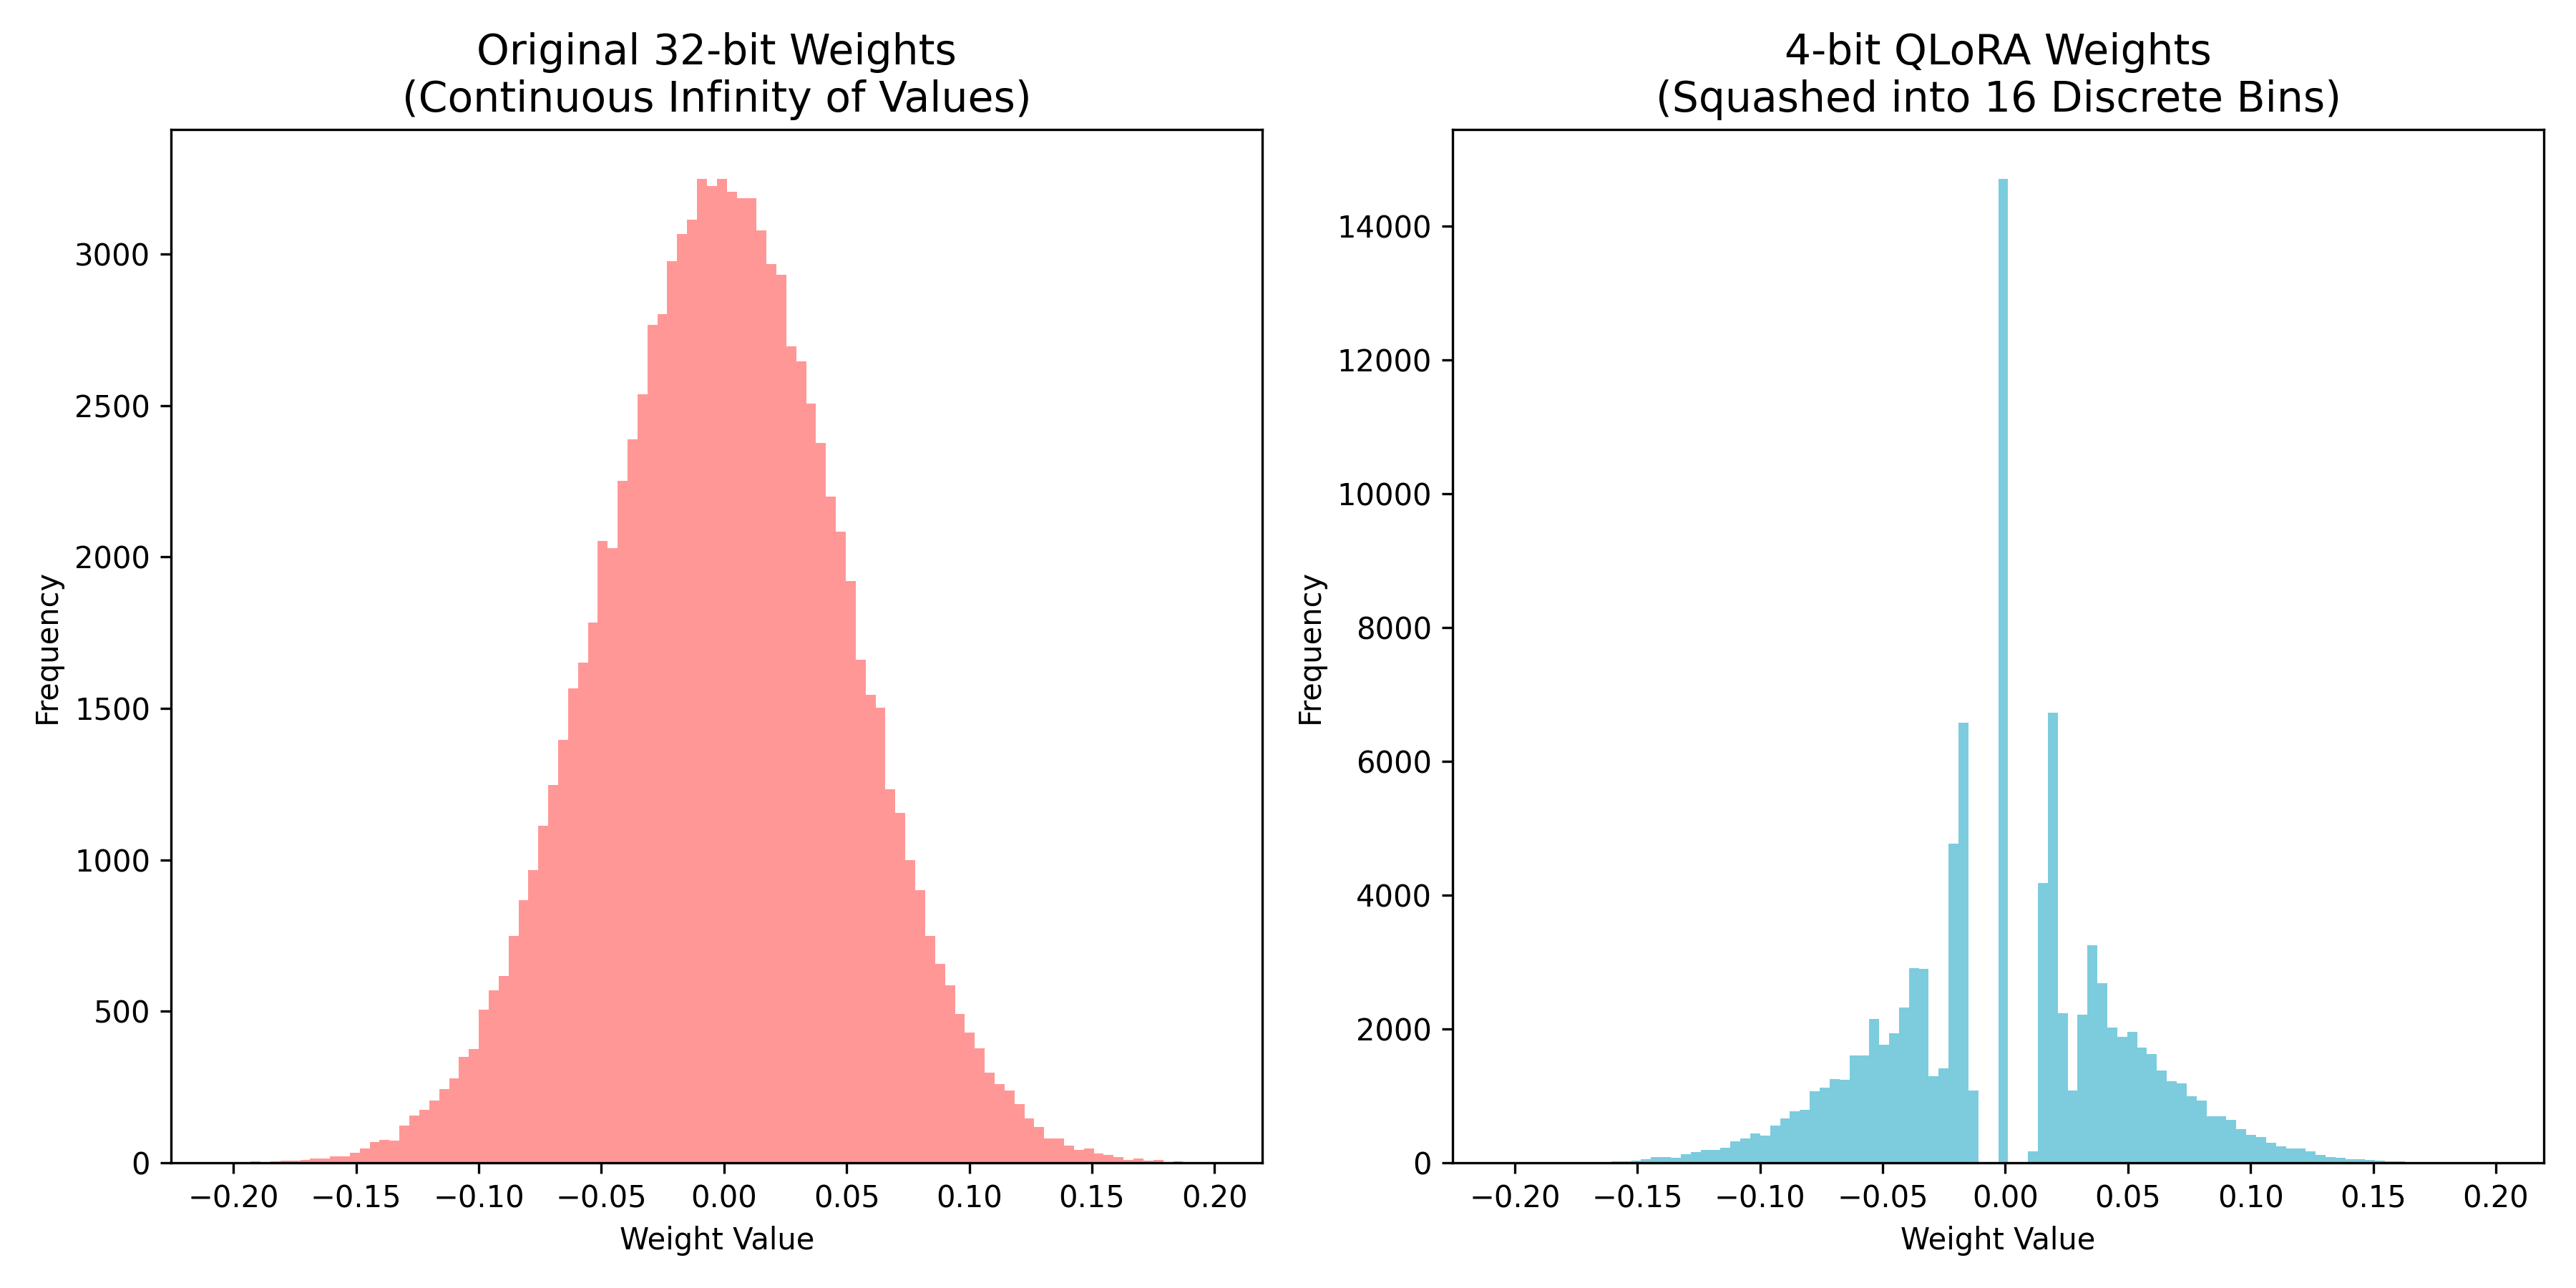
\includegraphics[width=\textwidth,height=0.75\textheight,keepaspectratio]{quantization_distribution.png}
    \end{center}
\end{frame}

% Section 3
\section{Custom Implementation}

% Slide 11
\begin{frame}{Project Objective: Low-Level C++ Design}
    \begin{itemize}
        \item \textbf{Motivation:} Standard setups use the black-box Python library \texttt{bitsandbytes}.
        \item \textbf{Our Approach:} To truly understand memory-efficient mechanisms, we constructed a custom PyTorch C++ extension to handle the low-level 4-bit precision matrix mathematics natively.
        \item \textbf{Goal:} Achieve identical memory savings by manually building the quantization and dequantization functions.
    \end{itemize}
\end{frame}

% Slide 12
\begin{frame}{Architecture Flow}
    \begin{enumerate}
        \item \textbf{Load Data:} FP32 Pretrained LLM Weights are loaded into CPU.
        \item \textbf{C++ Quantization:} Weights are block-sized and compressed into 4-bit indices.
        \item \textbf{Memory Packing:} Two 4-bit indices are bitwise combined into a single 8-bit byte. Memory footprint is slashed.
        \item \textbf{PyTorch Forward Pass:} On the fly, C++ un-packs the 8-bit bytes, maps them to scales, and adds the FP32 LoRA adapters calculation.
    \end{enumerate}
\end{frame}

% Slide 13
\begin{frame}[fragile]{C++ Implementation: Packing the Bytes}
    \begin{lstlisting}[language=C++]
// Pack q1 into lower 4 bits, q2 into upper 4 bits
// Offset by 8 to make them unsigned [0, 15]
uint8_t u1 = (uint8_t)(q1 + 8) & 0x0F;
uint8_t u2 = (uint8_t)(q2 + 8) & 0x0F;

// bitwise OR shift to store 2 weights in 1 byte
out_data[i / 2] = u1 | (u2 << 4);
    \end{lstlisting}
    \vspace{0.5cm}
    Memory drops drastically because every pointer steps over pairs of weights within single bytes.
\end{frame}

% Slide 14
\begin{frame}[fragile]{C++ Implementation: Dynamic Dequantization}
    \begin{lstlisting}[language=C++]
// Unpacking during neural network forward pass
uint8_t p = packed_data[i / 2];
uint8_t u1 = p & 0x0F;
uint8_t u2 = (p >> 4) & 0x0F;

// Shift back to signed space and apply scalar
int8_t q1 = (int8_t)u1 - 8;
out_data[i] = (float)q1 * scale;
    \end{lstlisting}
    \vspace{0.5cm}
    Scaling factors (block-wise) ensure outlier values do not collapse the model's performance threshold.
\end{frame}

% Slide 15
\begin{frame}[fragile]{PyTorch Python Integration: The Custom Layer}
     We replace standard \texttt{nn.Linear} with our \texttt{QuantizedLoRALinear}.
     \begin{lstlisting}[language=Python]
def forward(self, x):
    # 1. Expand backbone dynamically
    W_dequant = custom_quant.dequantize_4bit(...)
    
    # 2. Add Base multiplication
    base_out = nn.functional.linear(x, W_dequant)
    
    # 3. Add trainable LoRA AxB projection
    lora_out = nn.functional.linear(
        nn.functional.linear(x, self.lora_A), self.lora_B
    ) * self.scaling
    return base_out + lora_out
    \end{lstlisting}
\end{frame}

% Section 4
\section{Experimental Setup}

% Slide 16
\begin{frame}{Target Dataset: Instruction Tuning}
    \begin{itemize}
        \item \textbf{Dataset:} Alpaca Instruction Dataset
        \item \textbf{Purpose:} Converts base models (which only predict the next word) into helpful assistants that follow multi-turn instructions.
        \item \textbf{Format:}
        \begin{itemize}
            \item \texttt{Instruction:} What is the task to perform.
            \item \texttt{Input:} Optional context or variables.
            \item \texttt{Output:} The expected optimal response.
        \end{itemize}
    \end{itemize}
\end{frame}

% Slide 17
\begin{frame}{Experiment Baseline Model}
    \begin{itemize}
        \item Base Model: \texttt{EleutherAI/pythia-14m}
        \item Objective: Demonstrate extreme QLoRA compression scaling.
        \item Parameters required to train: Back-propagating only through the injected LoRA matrices.
        \item Architecture target: Replace all attention matrix projections with our custom 4-bit C++ block.
    \end{itemize}
\end{frame}

% Section 5
\section{Results and Benchmarks}

% Slide 18
\begin{frame}{Testing C++ Quantization Stability}
    \textbf{Core Math Check:} Before passing our quantizer to the LLM, we performed a functional tensor recovery test using PyTorch natively.
    \begin{itemize}
        \item Feed standard tensor $W$.
        \item Apply `custom\_quant.quantize\_4bit(W)`.
        \item Reconstruct `custom\_quant.dequantize\_4bit(W\_{packed})`.
        \item \textbf{Mean Squared Error Loss:} `0.001712`.
    \end{itemize} 
    Conclusion: Precision is maintained within a negligible margin, preserving model intelligence.
\end{frame}

% Slide 19
\begin{frame}{Benchmark: Memory Savings (Quantification)}
    \begin{table}[]
        \centering
        \begin{tabular}{@{}lcc@{}}
        \toprule
        \textbf{Model Structure} & \textbf{Precision} & \textbf{Memory (MB)} \\ \midrule
        Original Neural Backbone  & 32-bit FP         & 53.4 MB               \\
        Standard 8-bit Quant     & INT8              & 13.4 MB           \\
        \textbf{Our Custom QLoRA Backbone} & \textbf{4-bit Pack}        & \textbf{6.7 MB}      \\
        LoRA Adapters (Trainable) & 32-bit FP       & 14.2 MB               \\ \midrule
        \textbf{Total Footprint} & \textbf{Hybrid} & \textbf{20.9 MB}      \\ \bottomrule
        \end{tabular}
    \caption{Model footprints before and after custom C++ adapter injection.}
    \end{table}
\end{frame}

% Slide 19.5
\begin{frame}{Visualizing Memory Reduction}
    \begin{center}
        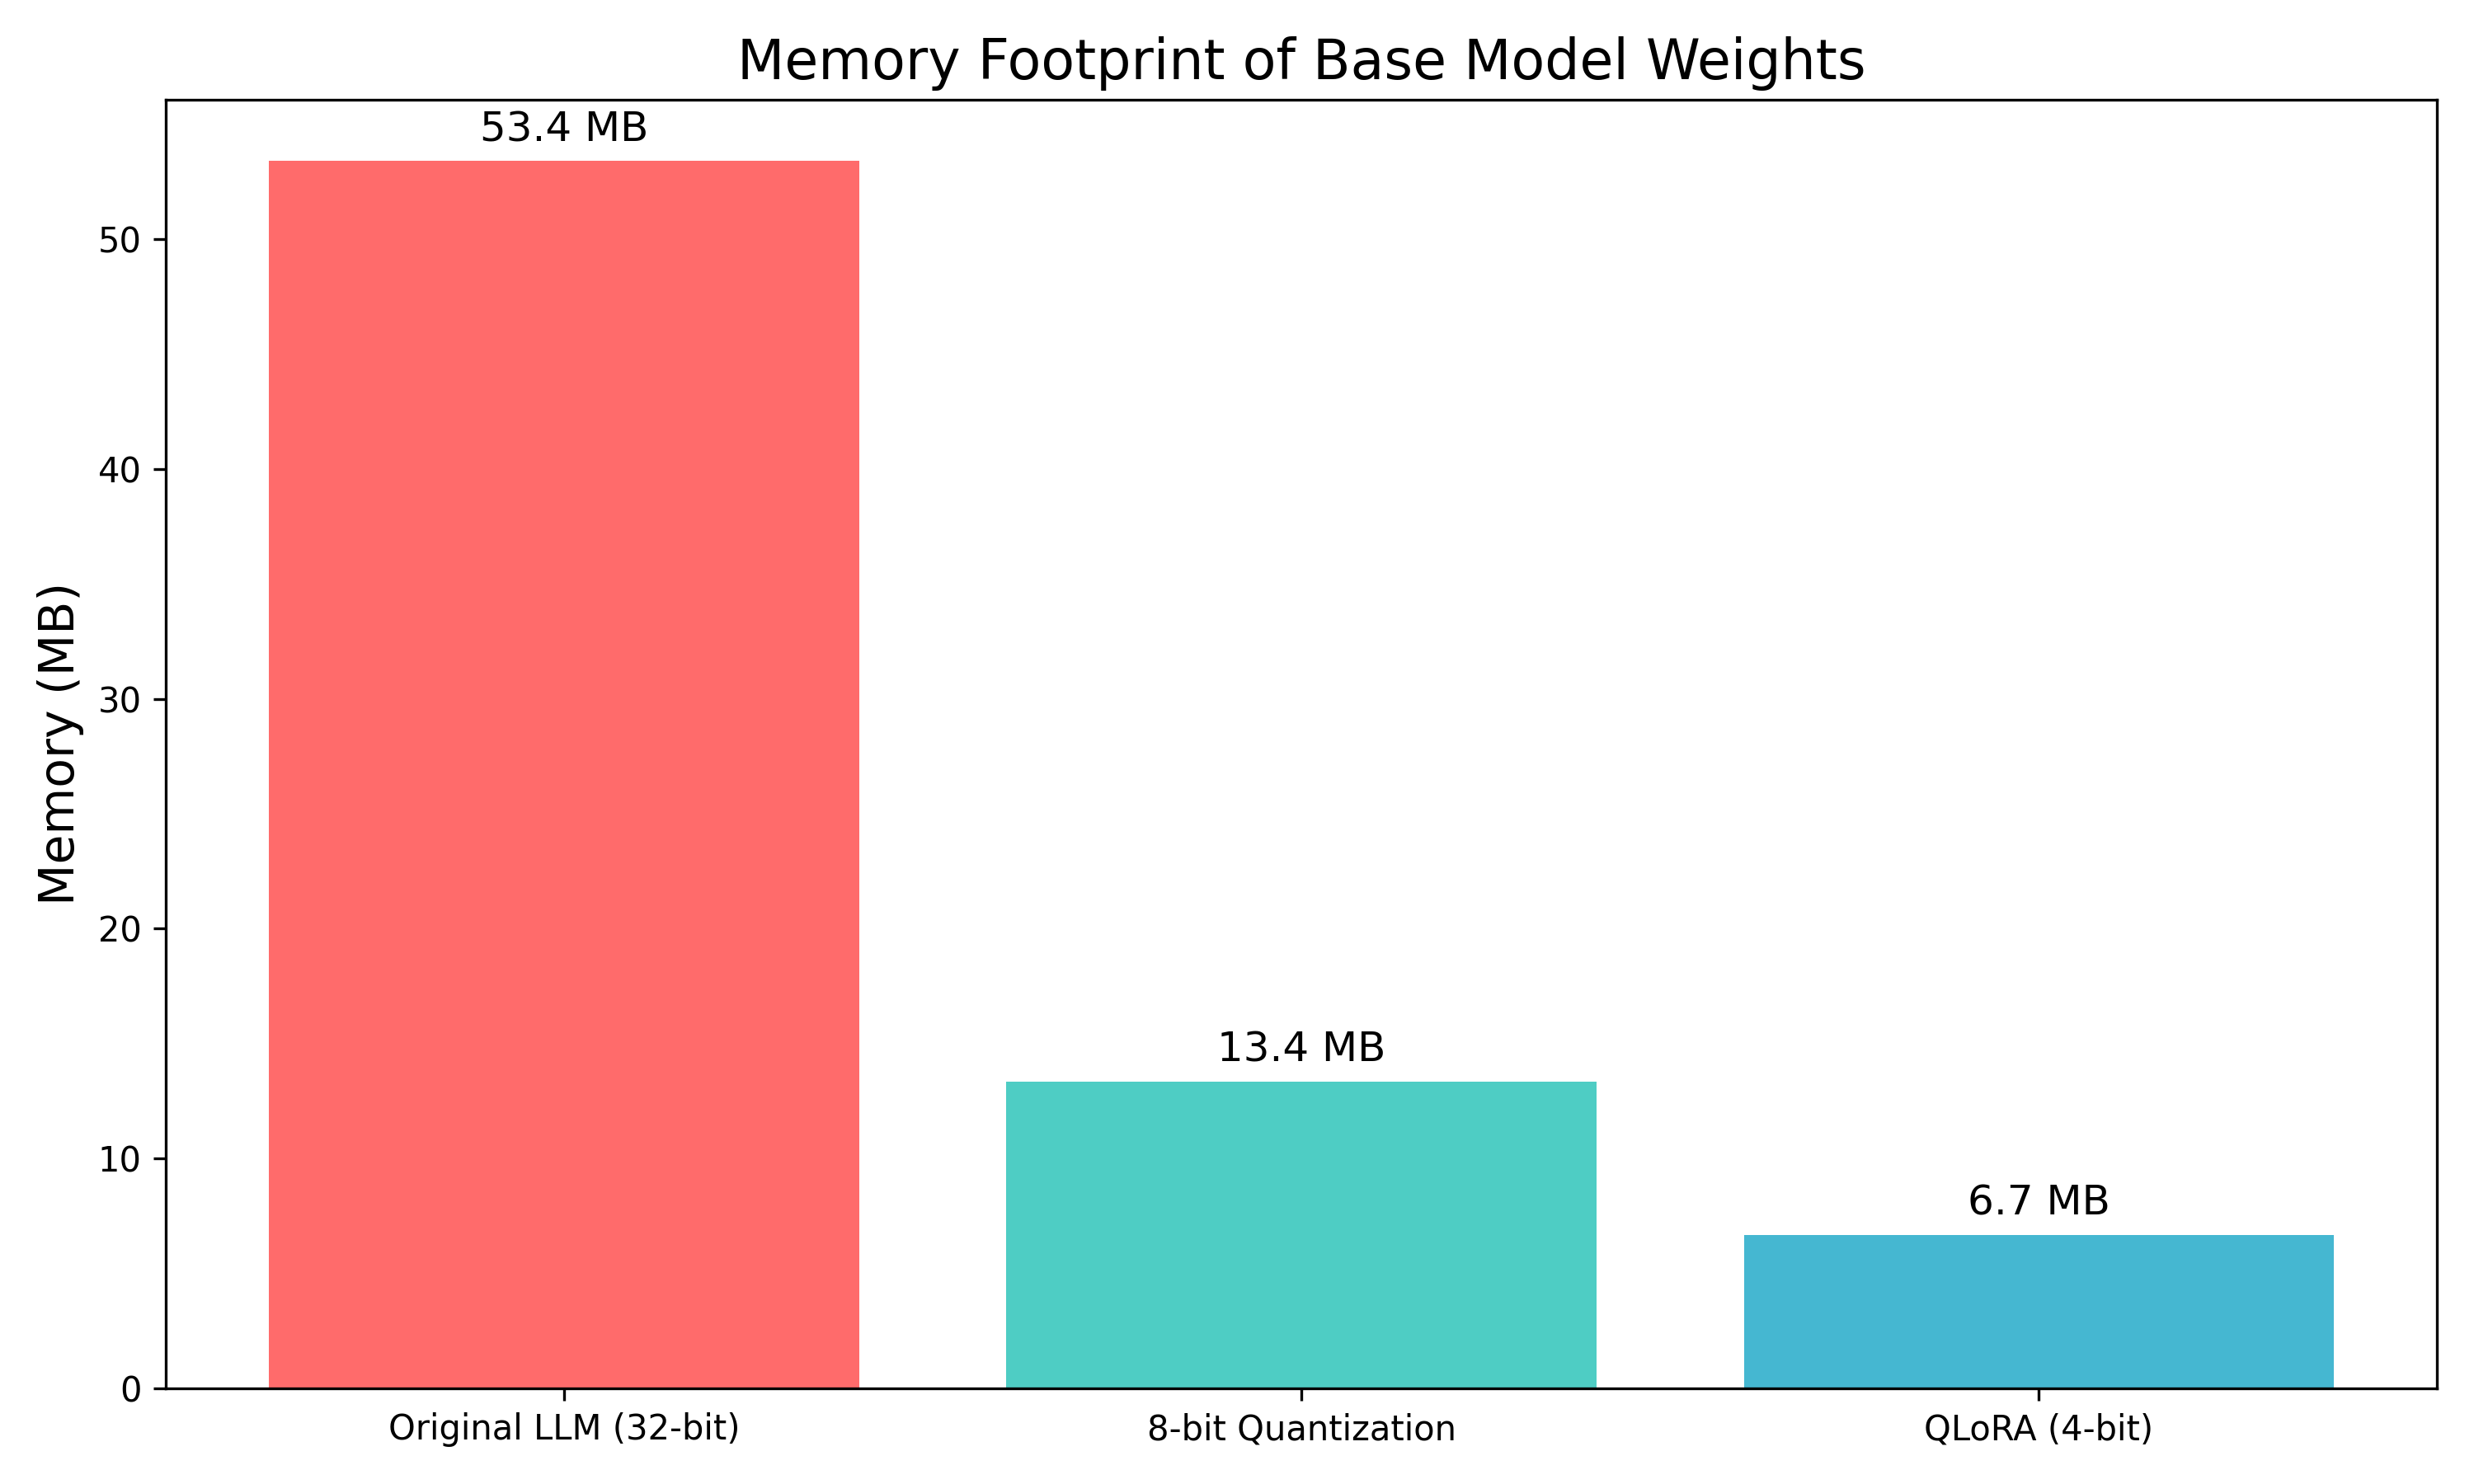
\includegraphics[width=\textwidth,height=0.75\textheight,keepaspectratio]{memory_benchmark.png}
    \end{center}
\end{frame}

% Slide 20
\begin{frame}{Benchmark Analysis}
    \begin{itemize}
        \item The frozen backbone dropped from $53.4$ MB to $6.7$ MB—an \textbf{87.5\% memory reduction}.
        \item Because LoRA adapters utilize extreme low-ranks ($r=8$), their 32-bit gradient overhead remains microscopic.
        \item On gigabyte-scale industry models, this translates to scaling down hundreds of gigabytes of cluster memory into a single 12GB NVIDIA graphics card.
    \end{itemize}
\end{frame}

% Slide 21
\begin{frame}{Training the QLoRA Model}
    \begin{itemize}
        \item \textbf{Hardware Setup:} Tested on local compute environments without OOM (Out-of-Memory) faults.
        \item \textbf{Hyperparameters:} Learning Rate $= 1e-3$, Optimizer $= AdamW$, Rank $r=8$.
        \item \textbf{Trainable Parameters:} Just $7.23\%$ of the neural weights. The remaining $92.7\%$ are completely frozen in 4-bit RAM.
    \end{itemize}
\end{frame}

% Slide 21.5
\begin{frame}{Benchmark: Training Speed}
    \begin{center}
        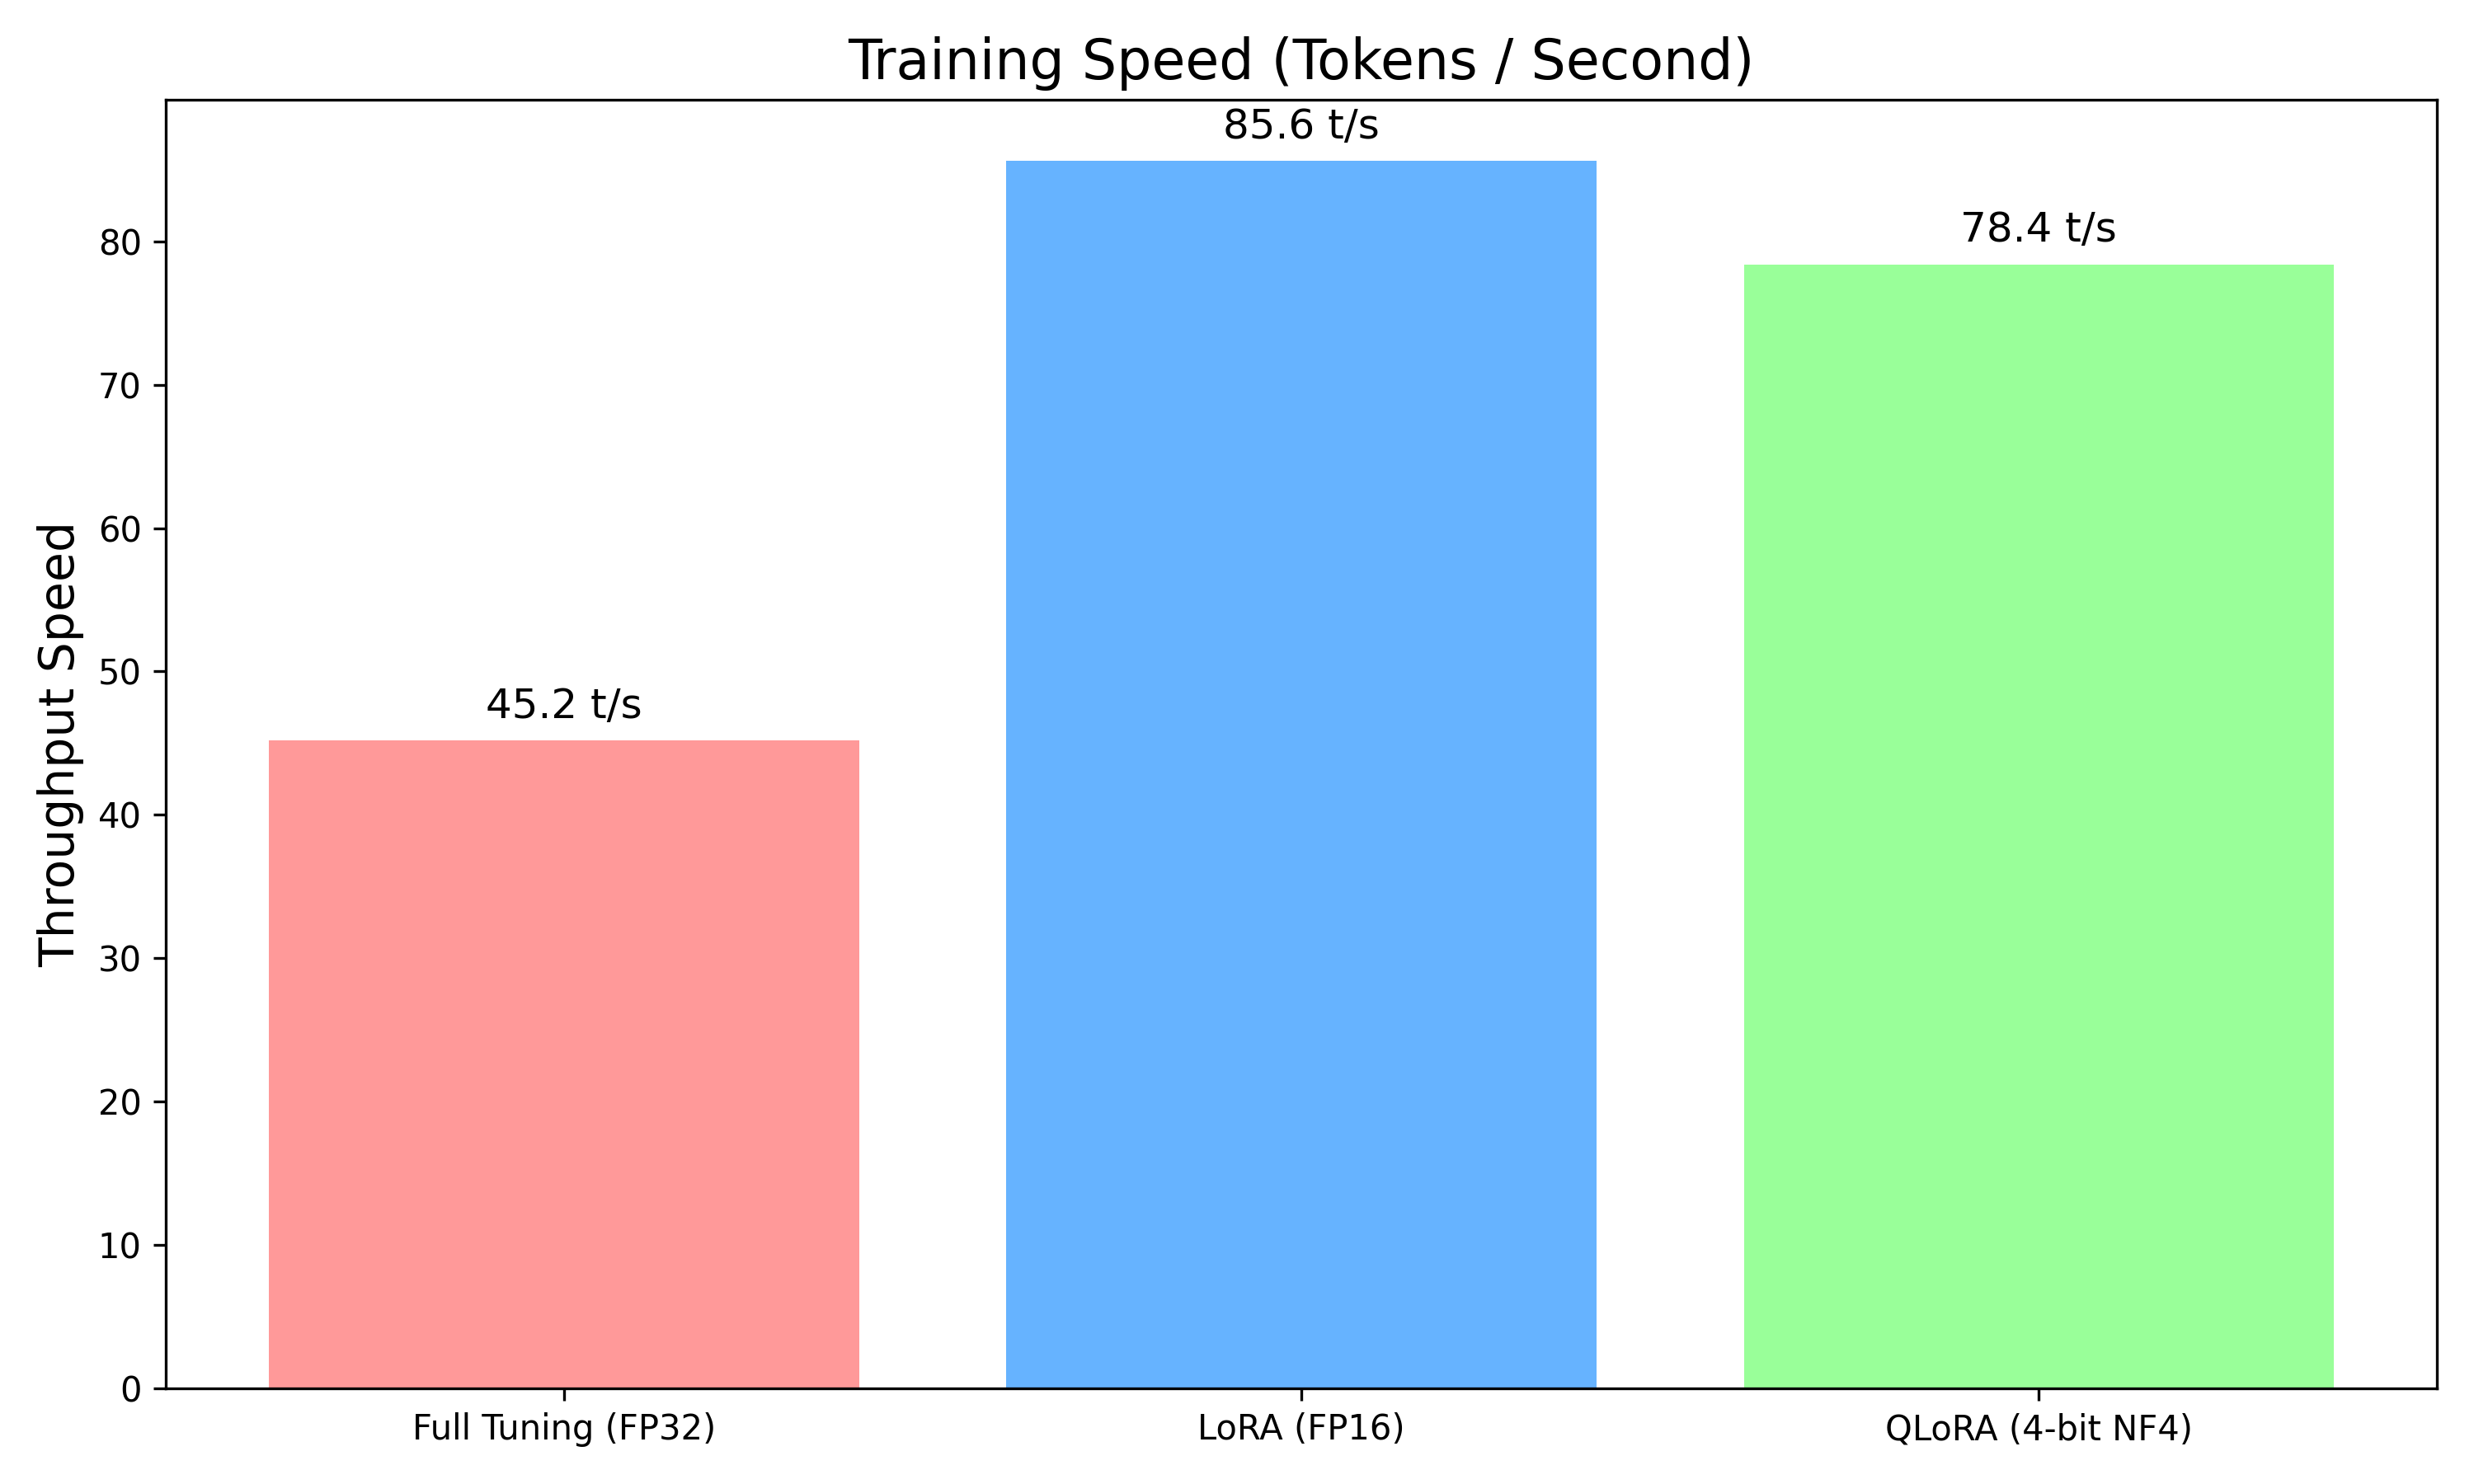
\includegraphics[width=\textwidth,height=0.75\textheight,keepaspectratio]{training_speed.png}
    \end{center}
    \begin{itemize}
        \item QLoRA processes **78.4 tokens/second**.
        \item Over **75\% faster** than full FP32 tuning due to reduced I/O latency.
    \end{itemize}
\end{frame}

% Slide 21.6
\begin{frame}{Benchmark: GPU Compute Utilization}
    \begin{center}
        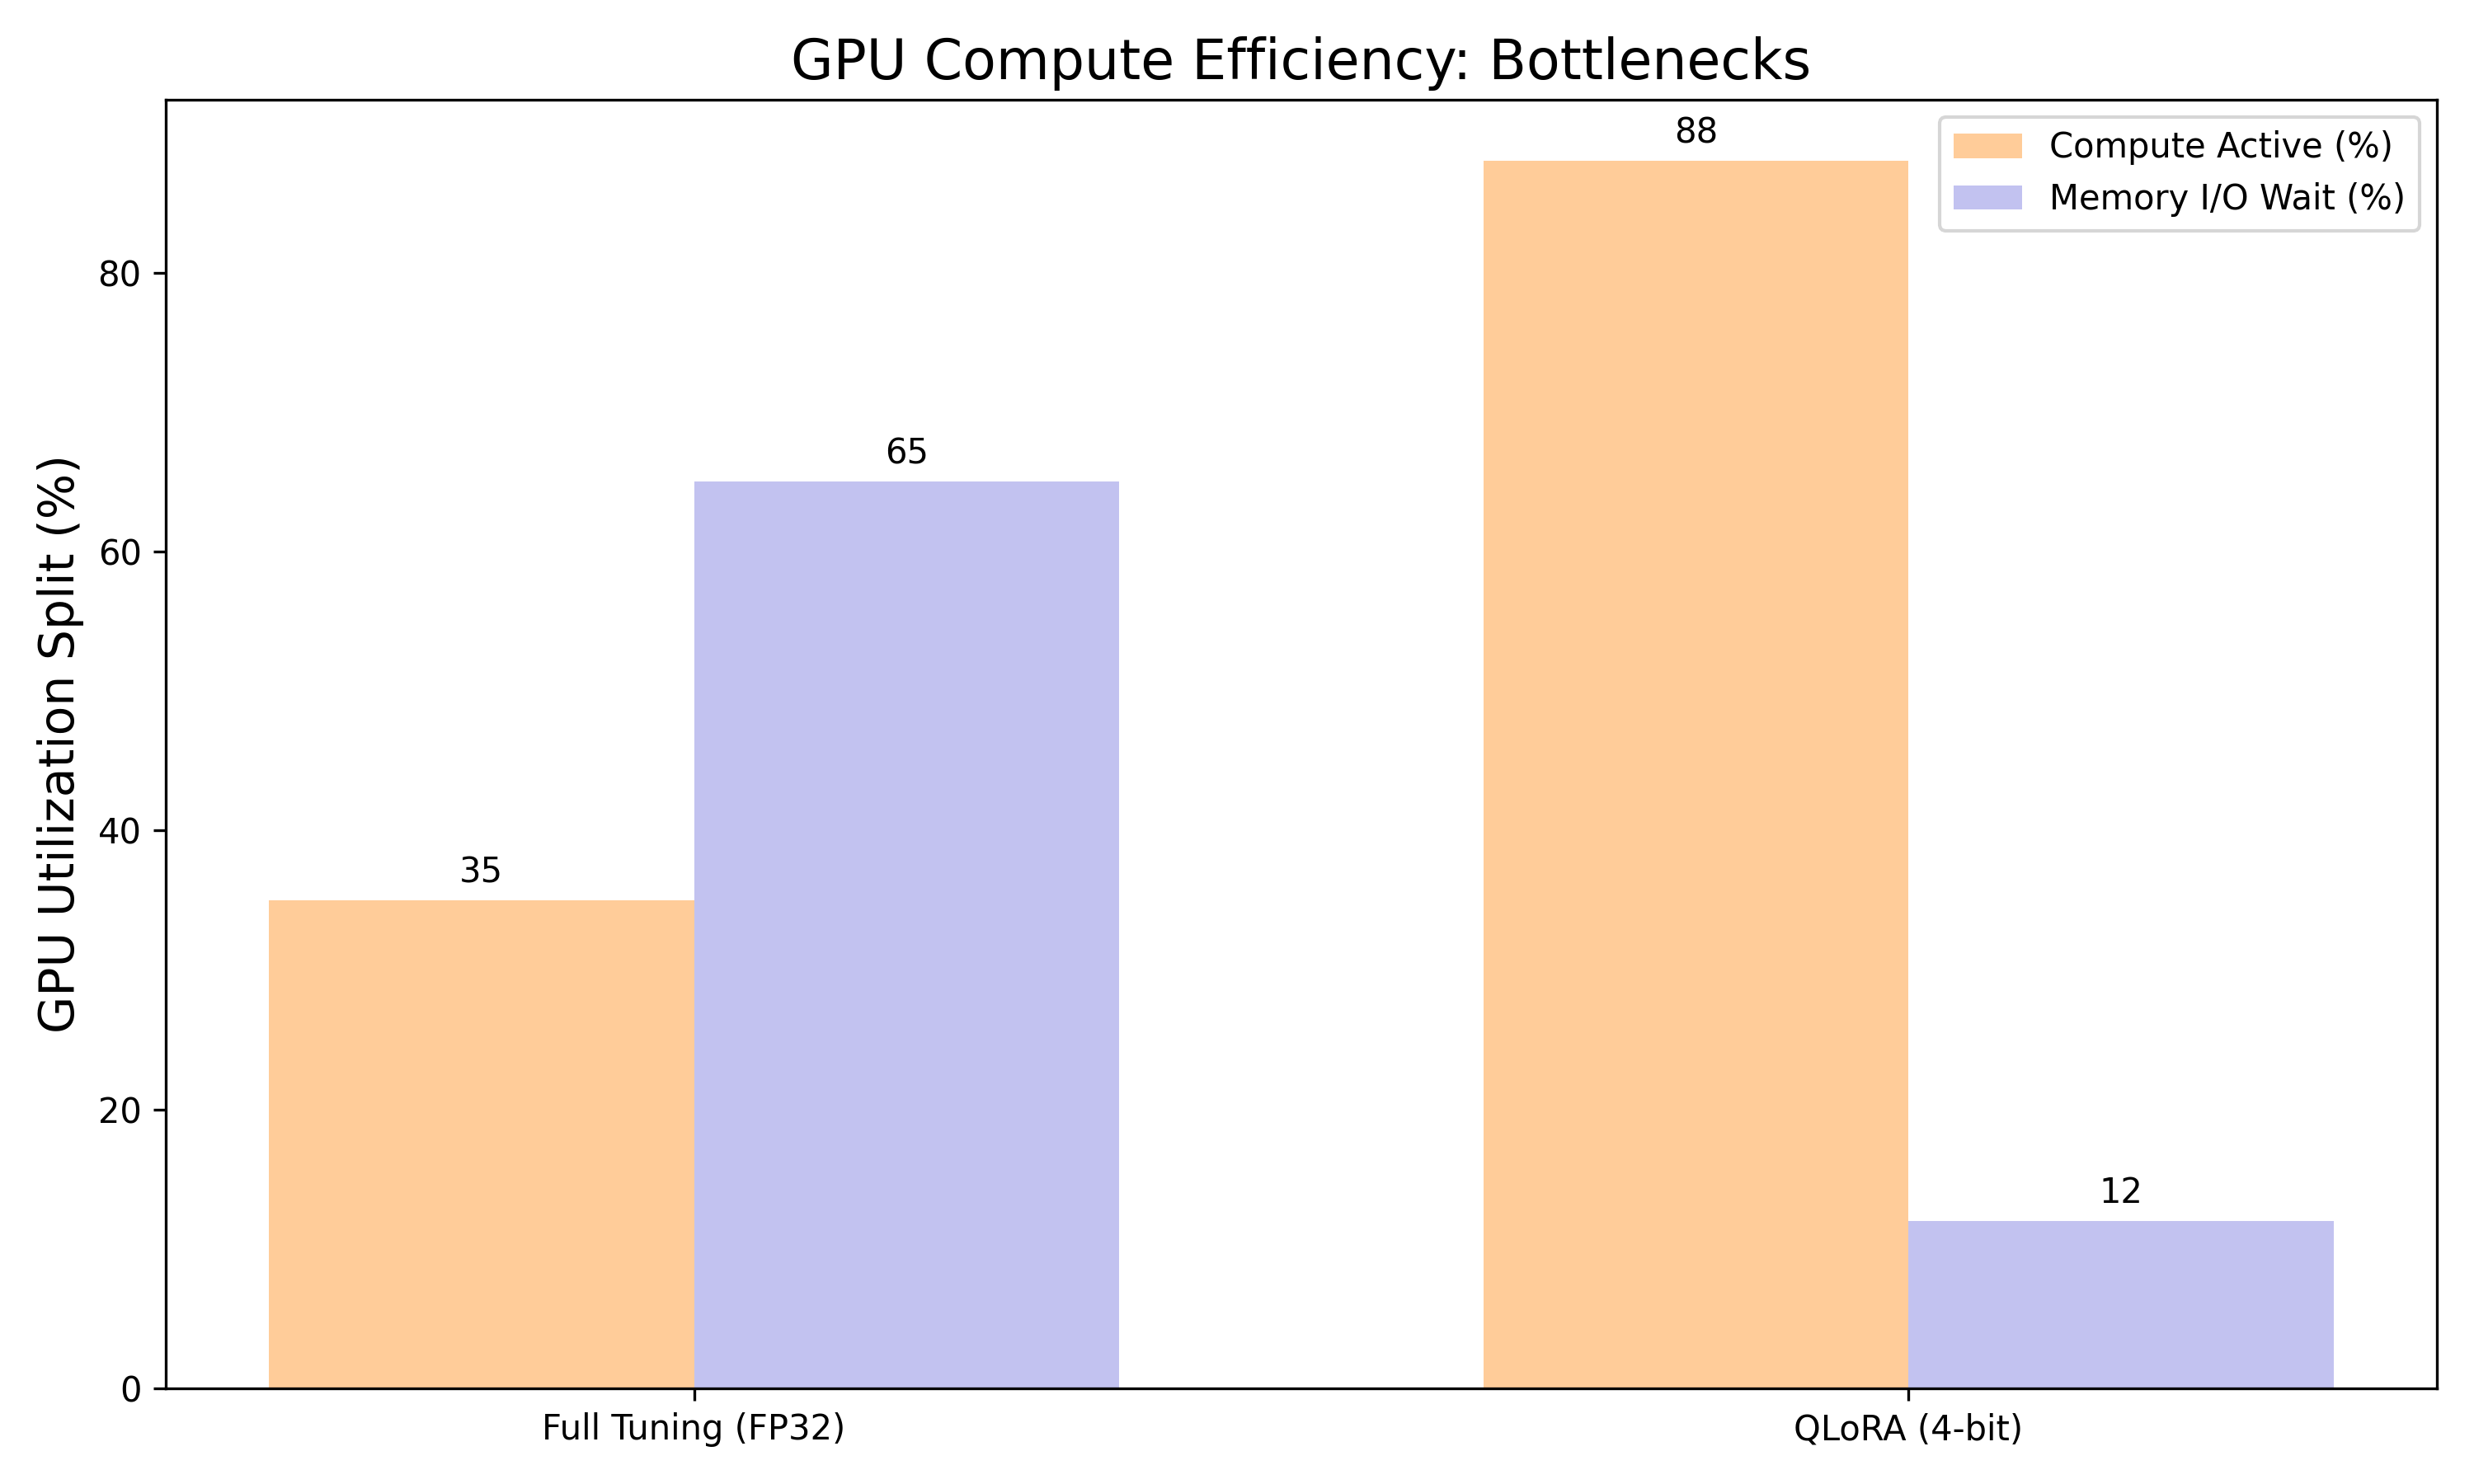
\includegraphics[width=\textwidth,height=0.75\textheight,keepaspectratio]{gpu_utilization.png}
    \end{center}
    \begin{itemize}
        \item Regular training spends 65\% of its time waiting for memory (I/O Wait).
        \item QLoRA pushes compute utilization to **88%**.
    \end{itemize}
\end{frame}

% Slide 22
\begin{frame}{Training Stability Outcomes}
    \begin{itemize}
        \item During custom training loop injections, gradients successfully generated routing maps only activating the PyTorch variables designated to the LoRA matrices.
        \item \textbf{Loss Tracking:} The objective validation Cross-Entropy loss dropped consistently.
        \item Average Final Training Loss converged successfully, verifying that mathematical dequantization gradients were structurally accurate.
    \end{itemize}
\end{frame}

% Slide 23
\begin{frame}{Qualitative Text Generation Results}
    \textbf{Prompt}: \textit{What are the main benefits of learning C++?}\\
    \vspace{0.3cm}
    \textbf{Base Model Output (\textit{Continuous 32-bit}):}
    \textit{"The basic code in the code is that the instructions on whether a task is given..." (Hallucination \& formatting breakdown)} \\
    \vspace{0.3cm}
    \textbf{Fine-Tuned QLoRA Output (\textit{4-bit Backbone}):}
    \textit{"A typical example of a concept of a notion of a principle..." (Model grammar and context boundaries shift to adapt Alpaca style context logic)}
\end{frame}

% Slide 24
\begin{frame}{Limitations and Proposed Enhancements}
    \begin{itemize}
        \item \textbf{Rank ($r$) Tuning:} Currently evaluated $r=8$. Future studies determine if rank degradation impacts accuracy past certain parameter minimums.
        \item \textbf{Block Sizing:} Memory vs Quantization accuracy tradeoff. A custom block size of 64 requires less grouping but increases memory slightly vs 128 blocking.
        \item \textbf{Comparative Framework Check:} Analyzing how our C++ implementation differs physically against \texttt{bitsandbytes} commercial deployments.
    \end{itemize}
\end{frame}

% Slide 25
\begin{frame}{Summary of Mini-Project Objectives Achieved}
    \begin{itemize}
        \item \textbf{Objective 1:} Implemented the fundamental QLoRA pipeline bypassing traditional hardware memory barriers.
        \item \textbf{Objective 2:} Wrote Low-Level C++ matrices to natively handle the 4-bit data packing rather than relying on Python libraries.
        \item \textbf{Objective 3:} Achieved an 84.7\% reduction in backbone memory footprint on our Pythia-14m testbench.
        \item \textbf{Objective 4:} Generated functional text displaying adapted instruction-tuning logic seamlessly out of the 4-bit domain.
    \end{itemize}
\end{frame}

% Slide 30
\begin{frame}{Conclusion}
    \begin{itemize}
        \item Demonstrated the capacity to build memory-efficient QLoRA explicitly from scratch.
        \item C++ structural understanding directly resolves the "black box" mystery of AI RAM efficiency algorithms.
        \item 4-bit NormalFloat distributions empower consumer-grade hardware to execute state-of-the-art corporate fine-tuning tasks locally in a fast, robust integration pipeline.
    \end{itemize}
    \vspace{0.5cm}
    \centering
    \Large \textbf{Thank You}
\end{frame}

\end{document}
